\documentclass[10pt, UKenglish]{beamer}
\usepackage{babel}
\usepackage[utf8]{inputenc}  
\usepackage{geometry}
\usepackage[customcolors]{hf-tikz}
\usepackage[T1]{fontenc}   
\usepackage{tcolorbox}
\usepackage{siunitx}
\usepackage{graphicx}
\usepackage{hyperref}
\usepackage{bookmark}
\usepackage{marvosym}
\usepackage{tikz}
\usepackage{tikz-qtree}
\usepackage{cancel}
\usepackage{todonotes}
\useoutertheme[subsection=false]{smoothbars}
\DeclareSIUnit[number-unit-product = {}]{\inchQ}{\textquotedbl}
\usepackage{amsmath,bm}
\DeclareSIUnit[number-unit-product = {\thinspace}]{\inch}{in}
\usetheme[menuwidth={0.3\paperwidth}]{erlangen}
\usepackage{multicol}
\usepackage{charter}
\setbeamercovered{transparent=20}
\setbeamertemplate{navigation symbols}{}
\sisetup{separate-uncertainty = true}
\usepackage[version=4]{mhchem}
\usepackage{tikz}
\usepackage{hepnames}
\usepackage{soul}
\usepackage{color}
\usepackage{thesis_defs}
\usepackage{subcaption}
\captionsetup[subfigure]{labelformat=empty}
\usepackage{xcolor}


\usepackage[backend=biber]{biblatex}
\bibliography{bibliography.bib}

\graphicspath{%
  {./feynman_diagrams/}%
  {./figures_theory/}%
  {./figures_simple/}%
  {./figures_misc/}%
  {./app1/}%
  {./app2/}%
  {./app3/}%
}


\definecolor{color1}{RGB}{33,217,217}
\definecolor{color2}{RGB}{7,61,111}

\newcommand{\lr}{\mathcal{lr}}


\newcounter{totavalue}
\newcounter{parvalue}

\def\aux{1}
\def\radius{9pt}
\def\step{4pt}
\usepackage[absolute,overlay]{textpos}


\newcommand\circcounter{%
\ifnum\inserttotalframenumber<2\relax
\else
  \setcounter{totavalue}{\inserttotalframenumber}
  \setcounter{parvalue}{\insertframenumber}
  \ifnum\inserttotalframenumber>45\relax
    \renewcommand\step{0pt}
  \fi%
  \pgfmathsetmacro{\aux}{360/3}
  \begin{tikzpicture}[remember picture,overlay, rotate=90+\aux]
  \foreach \i in {0,1,...,3}
    \fill[logo_blue] 
      (0,0) -- (-\i*\aux:\radius) arc  (-\i*\aux:-(\i+1)*\aux+\step:\radius) -- cycle;
  \foreach \i in {1,...,\insertframenumber}
    \fill[logo_grey] 
      (0,0) -- (-\i*\aux:\radius) arc  (-\i*\aux:-(\i+1)*\aux+\step:\radius) -- cycle;
  \fill[white] circle (\radius/1.3);
  \node at (0,0) {\small\insertframenumber}; 
  \end{tikzpicture}%
\fi%
}


\usepackage{eso-pic,picture}



\begin{document} 

\title[Neural network results in the dilep tau channel]{Neural network updates}
\subtitle{\today}
\author{Christian Kirfel}
%\institute{Universtität Bonn}
        



\begin{frame}[plain]
\vspace{0.0cm}
  \titlepage
      \AddToShipoutPictureFG*{%
    \AtPageUpperLeft{%
      \put(8.7cm,-9.6cm){

\includegraphics[scale=0.03]{original_logo.jpg}
\makebox(0,0)[lt]{}%
      }%
    }%
  }%
    \AddToShipoutPictureFG*{%
    \AtPageUpperLeft{%
      \put(0.0cm,-9.6cm){
%\includegraphics[scale=0.17]{atlas_gay.png}
%
\includegraphics[scale=0.17]{ATLAS-Logo-Ref-RGB-H_0.jpg}
\makebox(0,0)[lt]{}%
      }%
    }%
  }%
\end{frame}
\addtobeamertemplate{navigation symbols}{\vspace*{0.8cm}\hfill\circcounter\hspace*{0.7cm}}


\begin{frame}{Update Lepditau}
  \begin{columns}
    \begin{column}{0.5\textwidth}
      \includegraphics[width=0.95\textwidth]{/cephfs/user/s6chkirf/intnote/ANA-HIGG-2020-02-INT1/figures/lepditau_NN/loss.pdf}  
      \includegraphics[width=0.95\textwidth]{/cephfs/user/s6chkirf/intnote/ANA-HIGG-2020-02-INT1/figures/lepditau_NN/ROC.pdf}  
    \end{column}
    \begin{column}{0.5\textwidth}
      \includegraphics[width=0.8\textwidth]{/cephfs/user/s6chkirf/intnote/ANA-HIGG-2020-02-INT1/figures/lepditau_NN/signal_response.pdf}  
      \includegraphics[width=0.8\textwidth]{/cephfs/user/s6chkirf/intnote/ANA-HIGG-2020-02-INT1/figures/lepditau_NN/tZq_response.pdf}  
    \end{column}
  \end{columns}
\end{frame}


\begin{frame}{Update dileptau}
  \begin{columns}
    \begin{column}{0.5\textwidth}
      \includegraphics[width=0.95\textwidth]{/cephfs/user/s6chkirf/intnote/ANA-HIGG-2020-02-INT1/figures/dileptau_NN/loss.pdf}  
      \includegraphics[width=0.95\textwidth]{/cephfs/user/s6chkirf/intnote/ANA-HIGG-2020-02-INT1/figures/dileptau_NN/ROC.pdf}  
    \end{column}
    \begin{column}{0.5\textwidth}
      \includegraphics[width=0.8\textwidth]{/cephfs/user/s6chkirf/intnote/ANA-HIGG-2020-02-INT1/figures/dileptau_NN/signal_response.pdf}  
      \includegraphics[width=0.8\textwidth]{/cephfs/user/s6chkirf/intnote/ANA-HIGG-2020-02-INT1/figures/dileptau_NN/tZq_response.pdf}  
    \end{column}
  \end{columns}
\end{frame}








\end{document}